\documentclass[letterpaper, 11pt]{article}
\usepackage{comment} % enables the use of multi-line comments (\ifx \fi) 
\usepackage{fullpage} % changes the margin
\usepackage{fancyhdr} % for footer
\usepackage[UKenglish]{isodate}% http://ctan.org/pkg/isodate for date format
\usepackage[]{natbib}
\usepackage{hyperref}
\usepackage{graphicx}
\usepackage{wrapfig}
\usepackage[font={small,sf}]{caption}
\usepackage{epigrafica}%changes default font to epigrafica

\pagestyle{fancy}
\renewcommand{\headrulewidth}{0pt}

\lhead{}
\chead{}
\rhead{}
\lfoot{ENT 432 (Fall 2016) - Penn State}
\cfoot{}
\rfoot{\thepage}
\renewcommand{\footrulewidth}{0.4pt}
\title{Discover your inner Darwin: insect observation and collection}
\author{Open Entomology Project}
\def\labelitemi{--}

\begin{document}
\cleanlookdateon %removed ordinal date
\maketitle
\thispagestyle{fancy}

\section*{Background}
\begin{wrapfigure}{r}{0.5\textwidth}
  \vspace{-20pt}
  \begin{center}
    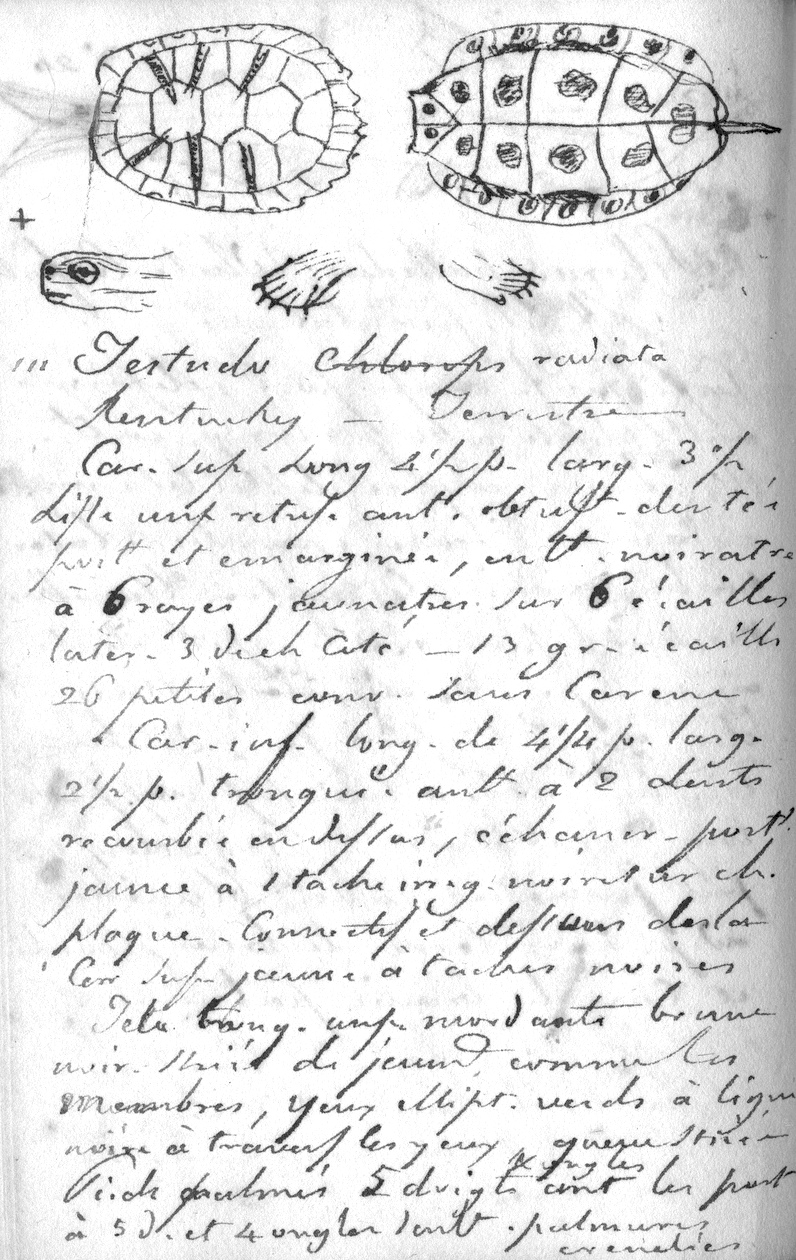
\includegraphics[width=0.38\textwidth]{Rafinesque}
  \end{center}
  \vspace{-16pt}
  \caption{A page from Constantine Rafinesque's (1818) field notebook. What would a page from yours look like? See original image: \url{https://flic.kr/p/dbEePV}}
  \vspace{-38pt}
\end{wrapfigure}
Entomology is informed, enriched, and inspired by a broad knowledge of natural history, what \cite{Tewksbury01042014} refer to as the ``fundamental properties of organisms''. We cover insect natural history extensively in lecture discussions and lab exercises---what insects eat, how they reproduce, how to diagnose taxa, how taxa are related, adaptations they have, how they interact with symbionts, parasites, predators, \textit{etc}. With respect to really understanding and appreciating insects, though, there is no substitute for time spent carefully observing these organisms in their natural environment and then in the lab, under the microscope. 

For this exercise you will spend time---at least 3 hours---carefully observing and documenting the insect life in a 4 m\textsuperscript{2} area. You will keep extensive field notes about what you see, and you will collect specimens that serve as vouchers for your observations and for the fauna represented in your area. This collection will be extended through subsequent collecting, the details of which are described below.

\section*{Your assignment}

\subsection*{Initial thoughts (20 pts.)}
Spend five or ten minutes observing an ant nest, a flower, a spider web, or some other natural object. If you had a pencil and paper what kinds of data would you be recording? What would you sketch? Now imagine that this exercise was extended into a deep, 3-hour (or longer) session, covering 4 m\textsuperscript{2}. Which habitat would you want to observe? What kinds of supplies and equipment would you need? Note that specialized collecting gear is available through the museum. Other questions to consider in your initial proposal:
\begin{itemize}
\item How would you choose your plot? What characteristics would you want it to have? How would you incorporate a temporal component? 
\item What are the minimum data you intend to record? How would a typical page in your notebook be organized?
\item How would you collect specimens and label them in a way that they could be associated with the observations you made in your journal? Be sure to read the Collection section below.
\item How would you account for the arthropod fauna you weren't able to observe directly? It's important that you sample your plot extensively, growing your collection beyond those few arthropods you spent time observing. 
\item Make a list of gear you need to bring.
\item Photos, recordings, and video are not required for these observations. If you do have digital content from these sessions how will you make those available for a broad audience and in a sustainable way?
\end{itemize}

\noindent{}Write your ideas out on a piece of paper, and discuss the approach with your fellow students. This original proposal should be turned in to your instructors. Don't worry if it's rough around the edges!

\subsection*{Refined thoughts (30 pts.)}
After discussing your approach with your classmates did you make any changes? Rewrite your thoughts into a proposal (two pages ought to cover it) that addresses the above questions. Turn this in by email, one week from today.

\subsection*{Field Notebook (100 pts.)}
The notebook serves as the record of your natural history observations. It likely will contain substantial data about insects, but it may also include sketches, thoughts, stories, hypotheses, notes about what to do in future observations, \textit{etc}. This component is a substantial portion of your grade for this exercise, and people will have free access to the final product. Any mistakes you make while writing must \textit{NOT} be erased. A single line through the error is sufficient to indicate a mistake. We allow for a more or less free flow of ideas, but we ask that each page follow some basic formatting: your name and the date in top corner of page, and the locality in top middle of each page.\\

\noindent{}We will provide you with a field notebook that is archival and water resistant (Rite In The Rain No: 371FX, 4 5/8 $\times$ 7$''$, 48 pages). \textit{This notebook is property of the Frost Entomological Museum and must be deposited there at the end of the semester.} You should use only pencil or an archival ink (\textit{e.g.}, Sakura\textregistered{ }Pigma Micron\textregistered; \url{http://www.pigmamicron.com/museums}); neither of these is provided. 

\subsection*{Collection (150 pts.)}
You should collect specimens for each kind of insect you observed in your plot, especially if they are the subject of content in your field notebook (\textit{i.e.}, they are vouchers for observations). You should also collect specimens of insects you \textit{didn't} see but know occurred in your plot. To complete your collection find specimens of 40 insect families that did \textit{not} occur in your plot, including 20 families we don't cover in lab.\\

\noindent{}Specimens must be determined minimally to family, and the collection should be accompanied by a spreadsheet. See the Collection Guidelines handout for more details regarding specimen preparation, labeling, and organization.

\subsection*{Synthesis and highlights (50 pts.)}
During your observation session(s) there was undoubtedly some insect that you found extraordinarily compelling. It exhibited unusual behavior, for example, or had some bizarre phenotype you want to know more about. You should take the relevant specimens, determine them to species, and then research the phenomenon that you found interesting. The results should be summarized in a narrative written for a broad audience---for example, something you would see on a blog---and include references, including the diagnostic tools you used, sketches, photos, \textit{etc}. Ask lots of questions and discuss your ideas with your instructors. Solicit feedback on your your narrative as it develops!

\section*{Further reading}
Numerous authors have highlighted the importance of natural history knowledge for the life sciences. \cite{agrawal2014} and \cite{wilcoveeisner2000} provide relatively simple yet compelling examples of the importance of insect observation. See also \cite{Schmidly449} and \cite{Barrows13042016} for discussions of natural history as part of the broader life sciences curriculum. For a celebration of field notes, including examples from ecologists, ethologists, systematists, and other scientists see \cite{canfield2011field}. Be sure also to peruse \cite{roberts2013} for a fascinating read on the effects of deep, patient observation.

% adding bibliography here
\bibliographystyle{apalike}
\bibliography{bib}
\end{document}

Given this paper - http://dx.doi.org/10.1093/biosci/biw043 - perhaps we need a natural history exercise.

(0) Student thinks about his/her background and interests. Based on these and a brief experiment (e.g., watch a spider web for 10 mins) s/he develops a proposed workflow or approach to observing and documenting insect natural history. What materials and supplies will s/he need? How will specimens be matched to observations in a notebook? What kinds of data will be collected? A proposal (1 pg) is written and given to a partner.

(1) Students vet each other's proposal and provide constructive feedback. A refined proposal is turned in for a grade.

(2) Instructors set up 4 m2 areas in different habitats. Students are told which ones they are to spend 4 hours observing/collecting/documenting the insects in it.

(3) Students are then told which one to move to for new observations.

(4) After 2 or 3 iterations student medidates on these observations, discusses them with partner, then chooses 2 or 3 (or 1?) observations s/he wants to develop knowledge on.

(5) The specimens from those key observations get determined to species, there is some literature search, and development of a presentation that is given eventually to the group.

(6) To complement this initial collection, which likely has low diversity relative to all possible insects that occur in PA, students dip into bulk samples taken from similar habitats (e.g., a Malaise trap set up in same meadow for a week). They each need to pull out insects that represent 20 families they didn't observe during their exercise.

(7) The entire collection and raw field notes are turned in, and the stories are presented to the class
